\documentclass[11pt, addpoints, answers]{exam}

\usepackage{amsmath, amssymb, amsthm}
\usepackage{xcolor}
\usepackage{graphicx}
\usepackage{graphics}
\usepackage{enumerate}


\usepackage{tikz}
\usepackage{tikz-qtree}
\usetikzlibrary{graphs}
\usetikzlibrary{arrows.meta}
\usepackage{listings}   
\usepackage{caption}
\makeatletter
\makeatother


\usepackage{algorithm}
\usepackage{algorithmic}




% For inserting code snippets.
\usepackage{listings}
\lstset{
	columns = fixed,
	basewidth = {0.5em},
	breaklines = true,
	backgroundcolor = \color{white},
	keywordstyle = \color[RGB]{40, 40, 255},
	numberstyle = \footnotesize\color{darkgray},
	commentstyle = \ttfamily\color{violet},
	basicstyle = \ttfamily,
	stringstyle = \ttfamily\color[RGB]{128, 0, 0},
	showstringspaces = false,
	language = {[11]C++},
	escapechar = \@
}
\lstnewenvironment{cpp}[1][]{\lstset{language = {[11]C++}, #1}}{}

\usepackage{tikz}

% headers, footers, titles
\newcommand{\CourseName}{CS101 Algorithms and Data Structures}
\newcommand{\HomeworkNO}{Homework 7}
\newcommand{\DueDate}{Due date: 23:59, November 13th, 2022}

\pagestyle{headandfoot}
\runningheadrule
\runningheader{\CourseName}{\HomeworkNO}{\DueDate}
\runningfooter{}{\thepage}{}

\title{
	\CourseName\\
	Fall 2022\\
	\HomeworkNO
}
\author{}
\date{\DueDate}

% formats of questions, choices, points, etc.
\qformat{\bf\thequestion. (\totalpoints\ points) \thequestiontitle\hfill}
\pointname{'}
\CorrectChoiceEmphasis{\bf\color{blue}}
\SolutionEmphasis{\color{blue}}

% We frequently use this font.
\newcommand{\ttt}{\texttt}

\begin{document}

\maketitle

\begin{enumerate}
	\item Please write your solutions in English.
	\item Submit your solutions to gradescope.com.
	\item Set your FULL name to your Chinese name and your STUDENT ID correctly in Account Settings.
	\item If you want to submit a handwritten version, scan it clearly. \ttt{CamScanner} is recommended.
	\item When submitting, match your solutions to the problems correctly.
	\item No late submission will be accepted.
	\item Violations to any of the above may result in zero points.
\end{enumerate}

\begin{questions}

	\titledquestion{Multiple Choices}

Each question has \textbf{one or more} correct answer(s). Select all the correct answer(s). For each question, you will get 0 points if you select one or more wrong answers, but you will get 1 point if you select a non-empty subset of the correct answers.

Write your answers in the following table.

%%%%%%%%%%%%%%%%%%%%%%%%%%%%%%%%%%%%%%%%%%%%%%%%%%%%%%%%%%%%%%%%%%%%%%%%%%%
% Note: The `LaTeX' way to answer a multiple-choices question is to replace `\choice'
% with `\CorrectChoice', as what you did in the previous questions. However, there are 
% still many students who would like to handwrite their homework. To make TA's work 
% easier, you have to fill your selected choices in the table below, no matter whether 
% you use LaTeX or not.
%%%%%%%%%%%%%%%%%%%%%%%%%%%%%%%%%%%%%%%%%%%%%%%%%%%%%%%%%%%%%%%%%%%%%%%%%%%

\begin{table}[htbp]
	\centering
	\begin{tabular}{|p{2cm}|p{2cm}|p{2cm}|p{6cm}|}
		\hline
		(a) & (b) & (c) \\
		\hline
		%%%%%%%%%%%%%%%%%%%%%%%%%%%%%%%%%%%%%%%%%%%%%%%%%%%%%%%%%%
		% YOUR ANSWER HERE.
		  BD  &  AC   &  C   \\
		%%%%%%%%%%%%%%%%%%%%%%%%%%%%%%%%%%%%%%%%%%%%%%%%%%%%%%%%%%
		\hline
	\end{tabular}
\end{table}

\begin{parts}
	\part[2] A problem in $\NP$ is $\NPC$ if:
	\begin{choices}
		\choice It can be reduced to another $\NPC$ problem in polynomial time.
		\CorrectChoice There exists a $\NPC$ problem which can be reduced to it in polynomial time.
		\choice It can be reduced to any other $\NP$ problem in polynomial time.
		\CorrectChoice Any other $\NP$ problem can be reduced to it in polynomial time.
	\end{choices}


	\part[2] Assuming that $\P\neq\NP$, which of the following problems are in $\NPC$?
	You may search the Internet for more information if you are unfamiliar with the problems.
	\begin{choices}
		\CorrectChoice \texttt{LONG-PATH}: $(G,s,t,k)$ Given an undirected graph $G$,
		determine whether there exists a simple path from \(s\) to \(t\) whose length is greater or equal to $k$.
		\choice \texttt{HALTING}: $(P,I)$ Given a compilable C++ program $P$ and the input $I$ for $P$,
		determine if $P$ runs infinitely on $I$.
		\CorrectChoice \texttt{4-SAT}: $\phi$ Given a CNF (conjunction normal form)
		where each clause is the disjunction of exactly 4 literals,
		determine whether $\phi$ is satisfiable.
		\choice \texttt{PRIME}: $n$ Given a positive integer $n$, determine whether it is a prime number.
	\end{choices}

	\part[2] For two decision problems $A$ and $B$, suppose that $A\leq_p B$.
	Which of the following statements are true?
	(Hint: there exists complexity classes that are strictly bigger than $\NP$)
	\begin{choices}
		\choice $A\in \P \implies B\in \P$
		\choice $A\in \NPC\implies B\not\in \NPC$.
		\CorrectChoice $B\in \P\implies A\in \P$.
		\choice $B\in \NPC\implies A\in \NPC$.
	\end{choices}

\end{parts}


	\newpage
	\titledquestion{Graph traversal}
Consider the following directed graph starting with A.

\centering
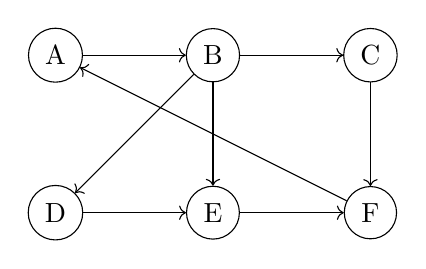
\begin{tikzpicture}[node distance=2cm]
    \node[circle, draw] (A) {A};
    \node[circle, draw, right of=A] (B) {B};
    \node[circle, draw, right of=B] (C) {C};
    \node[circle, draw, below of=A] (D) {D};
    \node[circle, draw, right of=D] (E) {E};
    \node[circle, draw, right of=E] (F) {F};

    \draw[->] (A) -- (B);
    \draw[->] (B) -- (C);
    \draw[->] (B) -- (D);
    \draw[->] (B) -- (E);
    \draw[->] (C) -- (F);
    \draw[->] (D) -- (E);
    \draw[->] (E) -- (F);
    \draw[->] (F) -- (A);
\end{tikzpicture}

\begin{parts}

\part[3]  Give the adjacency list for the graph. You should write the node in alphabetical order. (Leave it blank if the node has no neighbour)

\begin{align*} % Your solution here
    adj(A) =& [\underline{\qquad\qquad}],\\
    adj(B) =& [\underline{\qquad\qquad}],\\
    adj(C) =& [\underline{\qquad\qquad}],\\
    adj(D) =& [\underline{\qquad\qquad}],\\
    adj(E) =& [\underline{\qquad\qquad}],\\
    adj(F) =& [\underline{\qquad\qquad}],\\
\end{align*}


\part[3] Give the visited node order using the above adjacency list for Breadth First Search.
\begin{solution}
    
\end{solution}

\part[3] Give the visited node order using the above adjacency list for Depth First Search.
\begin{solution}
    
\end{solution}

\end{parts}
	\newpage
	\titledquestion{DSU on hand}[2]

\emph{I mean, hands on DSU, perhaps.}\\

Consider performing a series of merge opertions on a disjoint set structure employing union-by-height strategy.
Draw the resulting tree structure.\\
When merging two sets,
break tie by merging the tree whose root label is small into the other tree.

\newcommand{\SET}[1]{\{#1\}}

\begin{enumerate}[{\bf op} 1.]
	\item initialize: $\SET{1}, \SET{2}, \SET{3}, \SET{4}, \SET{5}, \SET{6}, \SET{6}, \SET{7}, \SET{8}$
	\item merge 1,8
	\item merge 2,7
	\item merge 3,6
	\item merge 4,5
	\item merge 1,4
	\item merge 2,3
	\item merge 5,3
\end{enumerate}

\begin{solution}
	% Give tikz-qtree a try!\\
	\vspace{60ex}
	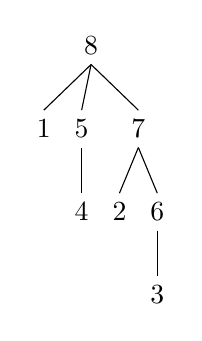
\begin{tikzpicture}
		\Tree [.8
				1
				[
					.5
					4
				]
				[.7
					2
					[
						.6
						3
					]
				]
		]
	\end{tikzpicture}
\end{solution}

	\newpage
	\titledquestion{The highest DSU I've ever seen}

In the following tasks, you can label the nodes by whatever mark you want.
We only care about the tree structure.

\begin{parts}
	\part[2] Plot a union tree of $15$ nodes with minimum height.
	The tree was generated by disjoint-set-union with union-by-height.\\
	\part[2] Plot a union tree of $16$ nodes with maximum height.
	The tree was generated by disjoint-set-union with union-by-height.\\
\end{parts}

\begin{solution}

for (a)\\\\

\begin{enumerate}[(a)]
%		\item Why not tikz?\\
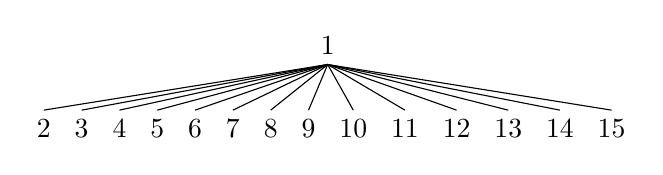
\begin{tikzpicture}
	\Tree [.1
		2 3 4 5 6 7 8 9 10 11 12 13 14 15
	]
\end{tikzpicture}
\end{enumerate}


for (b)\\\\
\begin{enumerate}[(b)]
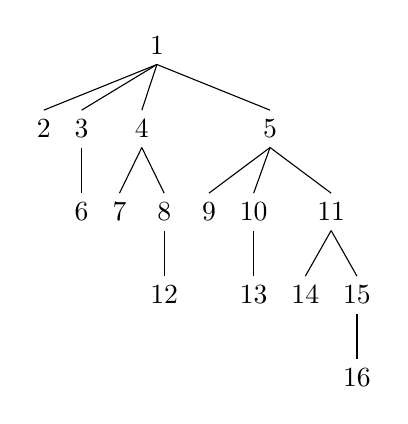
\begin{tikzpicture}
	\Tree [.1
		2
		[
			.3
			6
		]
		[
			.4
			7
			[
				.8
				12
			]
		]
		[
			.5
			9
			[
				.10
				13
			]
			[
				.11
				14
				[
					.15
					16
				]	
			]
		]
	]
\end{tikzpicture}
\end{enumerate}
%Also checkout mathcha.


\vspace{80ex}
\end{solution}



\end{questions}

\end{document}
